\documentclass{article}
\usepackage{tikz}
\usepackage{adjustbox}

\begin{document}

\begin{center}
    {\ttfamily \textbf{UNITED STATES}} \\
    {\ttfamily \textbf{AIR STATUS DISPLAY}}
\end{center}

\vspace{1em}

{\ttfamily \textbf{Date of}} \\
{\ttfamily \textbf{Mission}}

\begin{adjustbox}{center}
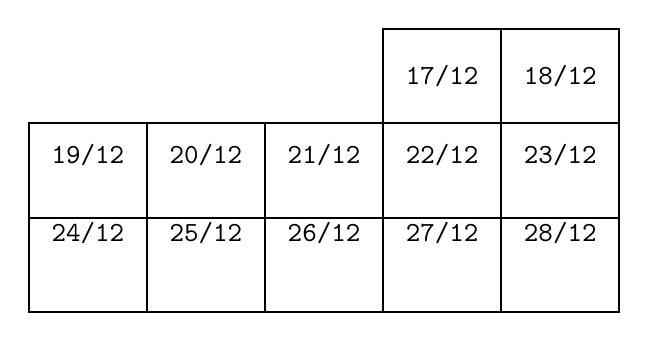
\begin{tikzpicture}
    % Define box size
    \def\boxwidth{1.5}
    \def\boxheight{1.2}

    % First row (top two boxes)
    \draw[thick] (3*\boxwidth, 0) rectangle (3*\boxwidth + \boxwidth, -\boxheight);
    \node at (3*\boxwidth + 0.75, -0.6) {\ttfamily \textbf{17/12}};

    \draw[thick] (4*\boxwidth, 0) rectangle (4*\boxwidth + \boxwidth, -\boxheight);
    \node at (4*\boxwidth + 0.75, -0.6) {\ttfamily \textbf{18/12}};

    % Second row (middle row)
    \foreach \x [count=\i] in {19, 20, 21, 22, 23} {
        \pgfmathsetmacro\xpos{\i - 1}
        \draw[thick] (\xpos*\boxwidth, -\boxheight) rectangle (\xpos*\boxwidth + \boxwidth, -2*\boxheight);
        \node at (\xpos*\boxwidth + 0.75, -1.6) {\ttfamily \textbf{\x/12}};
    }

    % Third row (bottom row)
    \foreach \x [count=\i] in {24, 25, 26, 27, 28} {
        \pgfmathsetmacro\xpos{\i - 1}
        \draw[thick] (\xpos*\boxwidth, -2*\boxheight) rectangle (\xpos*\boxwidth + \boxwidth, -3*\boxheight);
        \node at (\xpos*\boxwidth + 0.75, -2.6) {\ttfamily \textbf{\x/12}};
    }

\end{tikzpicture}
\end{adjustbox}

\end{document}
